% Chapter 11

\chapter{Results} % Chapter title

\label{ch:results} 

The results of the search can be seen in \autoref{tab:results}, which displays the expected and observed numbers of events in SRZ, both divided by channel and inclusively. The predictions and uncertainties for each background are shown, though many of these uncertainties are correlated between backgrounds, so the final uncertainty does not correspond to a simple addition in quadrature of each error. A total of sixty events are observed, with 53.5 $\pm$ 9.3 events expected. \autoref{fig:results_plot} shows the expected and observed results visually for the \ac{SR} as well as three \acp{VR}, all designed to verify the accuracy of the backgrounds taken from \ac{MC}. Excellent agreement is seen in all cases, with the largest deviation at about $1\sigma$. 

\begin{centering}
\begin{figure}[!hbt]
\myfloatalign
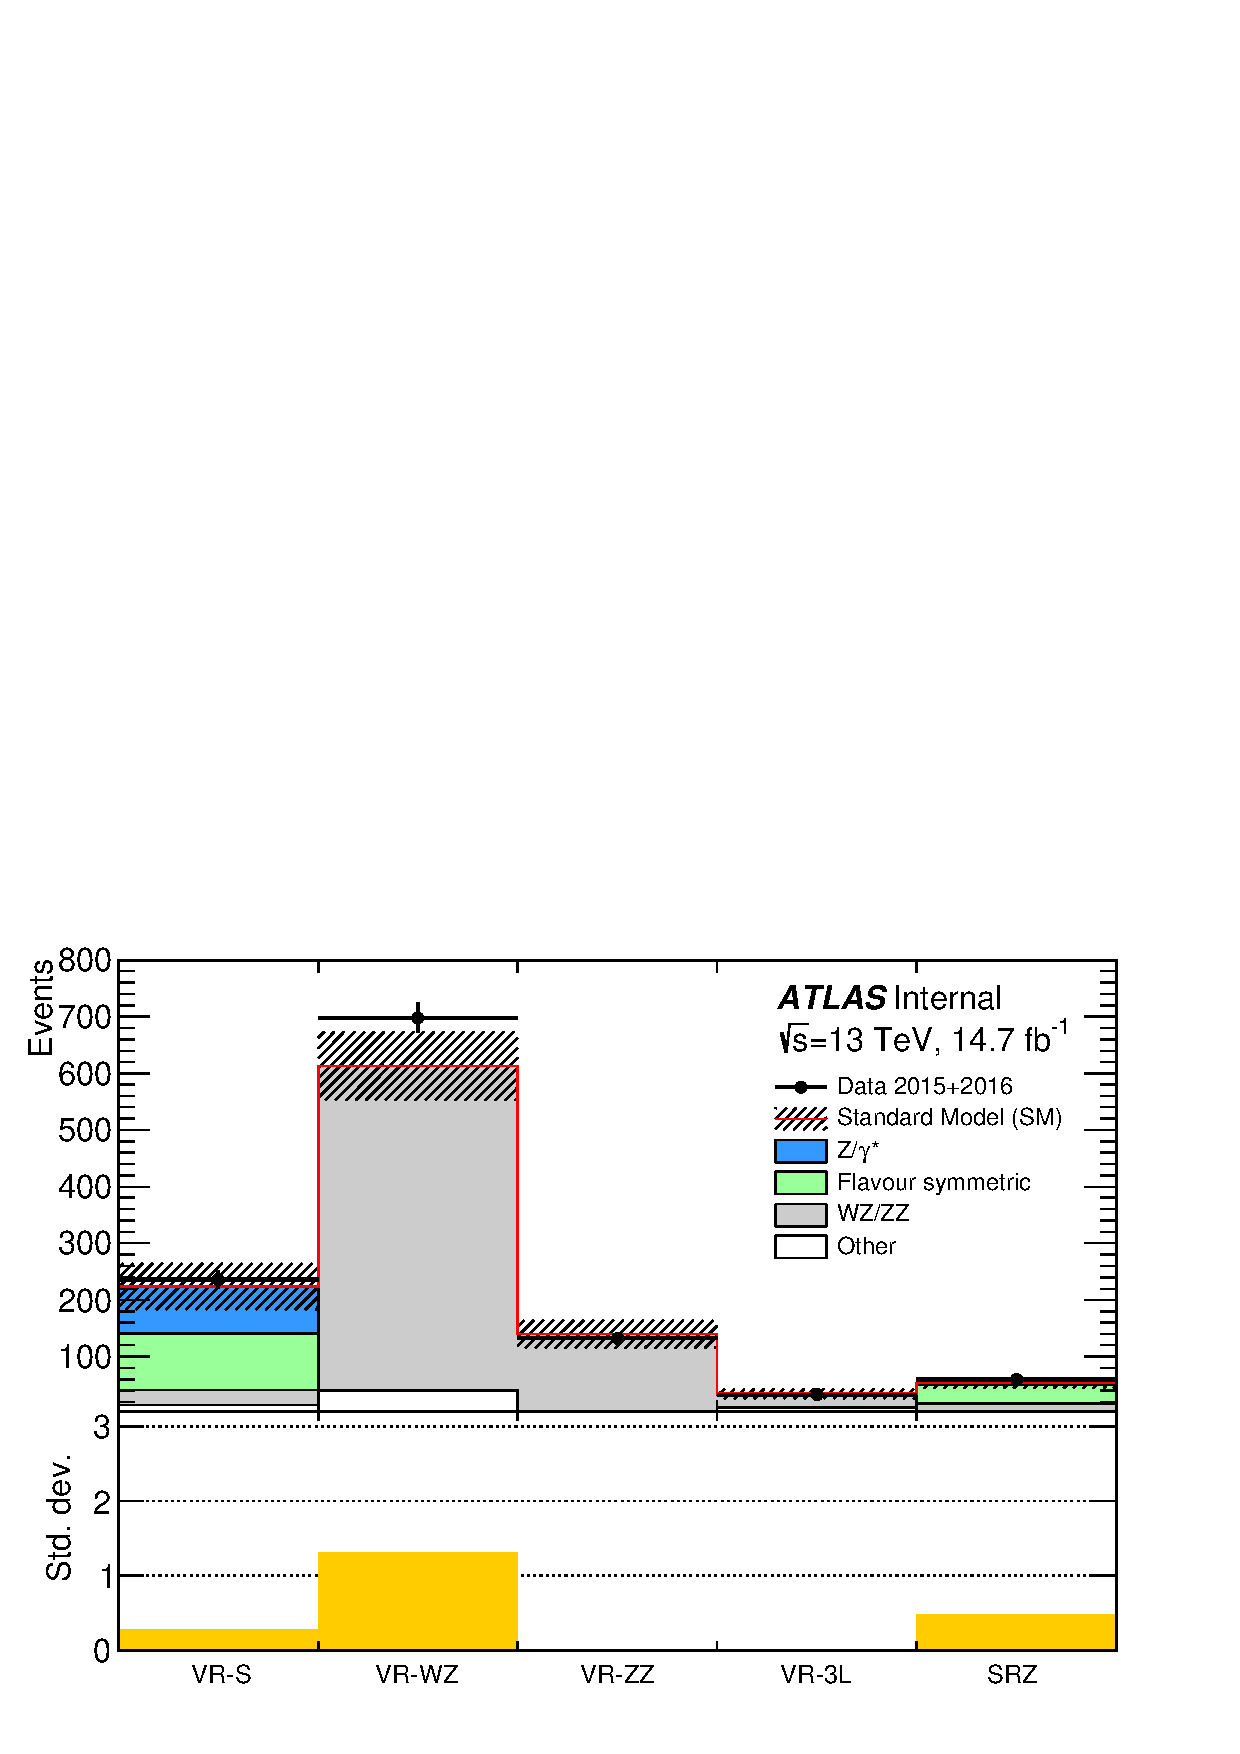
\includegraphics[width=.9\linewidth]{figures/results/makeSummaryPlot_linear.pdf}
\caption{Comparison of background predictions and data yields in four validation regions, as well as the signal region. Definitions of all regions can be found in \autoref{tab:regions-z}, with both rare top and fake backgrounds grouped together under the ``other'' label. The uncertainty band includes all statistical and systematic uncertainties. Below is a panel of the one-sided statistical significances of the deviations between the predicted and observed quantities for each region.}
\label{fig:results_plot}
\end{figure}
\end{centering}

\begin{sidewaystable*}
\caption{
Number of events expected and observed in the $ee$, $\mu\mu$, and combined channels. Expected predictions include all systematic and statistical uncertainties discussed in \autoref{ch:background_uncertainties}. Also shown is the discovery $p$-value for zero signal strength ($p(s=0)$)~\cite{Baak:2014wma}, Gaussian significance, 95\% \ac{CL} observed and expected upper limits on the number of signal events ($S^{95}$), and the corresponding observed upper limit on the visible cross section ($\langle\epsilon\sigma\rangle^{95}_\text{obs}$).
}
\begin{center}
\setlength{\tabcolsep}{0.0pc}
%%
\begin{tabular*}{\textwidth}{@{\extracolsep{\fill}}lccc}
\noalign{\smallskip}\hline\noalign{\smallskip}
                                                                            & SRZ                 & SRZ $ee$      & SRZ $\mu\mu$  \\[-0.05cm]
\noalign{\smallskip}\hline\noalign{\smallskip}
%%
Observed events                                                             & $60$                     & $35$                   &   $25$ \\
\noalign{\smallskip}\hline\noalign{\smallskip}
%%
Total expected background events                                            & $53.5 \pm 9.3$         & $27.1 \pm 5.1$       &   $26.8 \pm 4.4$ \\
\noalign{\smallskip}\hline\noalign{\smallskip}
%%
  Flavour-symmetric (\ttbar, $Wt$, $WW$ and $Z\rightarrow\tau\tau$) events  & $33.2 \pm 3.9$         & $16.5 \pm 2.1$       &   $16.7 \pm 2.0$       \\
%%
  \dyjets\ events                                                           & $\makebox[3ex]{\hfill 3.1} \pm \makebox[2ex]{2.8\hfill}$          & $1.0_{-1.0}^{+1.3}$ &   $\makebox[3ex]{\hfill 2.1} \pm \makebox[2ex]{1.4\hfill}$     \\
%%
  $WZ/ZZ$ events                                                            & $14.2 \pm 7.7$         & $\makebox[3ex]{\hfill 7.8} \pm \makebox[2ex]{4.3\hfill}$        &   $\makebox[3ex]{\hfill 6.4} \pm \makebox[2ex]{3.5\hfill}$        \\
%%
  Rare top events                                                           & $\makebox[3ex]{\hfill 2.9} \pm \makebox[2ex]{0.8\hfill}$          & $\makebox[3ex]{\hfill 1.4} \pm \makebox[2ex]{0.4\hfill}$        &   $\makebox[3ex]{\hfill 1.5} \pm \makebox[2ex]{0.4\hfill}$  \\
%%
 Fake-lepton events                                                         & $\makebox[3ex]{\hfill 0.1}_{-0.1}^{+0.8}$   & $0.5_{-0.5}^{+0.7}$ &   $\makebox[3ex]{\hfill 0}^{+0.2}$    \\
 \noalign{\smallskip}\hline\noalign{\smallskip}
$p(s=0)$                                                                    & 0.32      & 0.15        & 0.5        \\
Significance $(\sigma)$                                                               & 0.47                     & 1.00                   & 0           \\
Observed (Expected) $S^{95}$                                                & 28.2 ($24.5_{-6.7}^{+8.9}$) & 22.0 ($15.8_{-4.5}^{+6.5}$) & 12.9 ($14.0_{-3.9}^{+5.7}$) \\
$\langle\epsilon\sigma\rangle^{95}_\text{obs}$~[fb]                         & 1.9             & 1.5                    & 0.88   \\
 \noalign{\smallskip}\hline\noalign{\smallskip}
\end{tabular*}
\end{center}
\label{tab:results}
\end{sidewaystable*}

\autoref{tab:results} also shows several statistical interpretations of the results. The discovery $p$-value for zero signal strength, which gives the probability that the observed events are compatible with a \ac{SM}-only hypothesis, is given as 0.32. The significance is listed as 0.47 $\sigma$, which is a reinterpretation of the $p$-value into a gaussian significance. This $p$-value is one-sided; when the data yield is less than expected the $p$-value is set to 0.5, and the significance is set to 0. $S^{95}$, the upper limit on the number of signal events that could be in the \ac{SR} at a 95\% \ac{CL}, is determined both for the expected and observed number of events. This limit is also reinterpreted based on the integrated luminosity used in the seach to produce an upper limit on the visible cross-section of signal events, $\langle\epsilon\sigma\rangle^{95}_\text{obs}$.

The predictions in SRZ, combined with \mll~shapes taken from \ac{MC}, are used to produce plots in a broader \mll~range, seen in \autoref{fig:results_widemll}. These plots are useful demonstrations of efficacy of the background estimation methods, showing the well-modeled \dyjets shape in the same-flavor region, and in the different-flavor region, demonstrating that there are no extreme fluctuations within the region used to predict the flavor symmetric background.

\begin{centering}
\begin{figure}[!hbt]
\myfloatalign
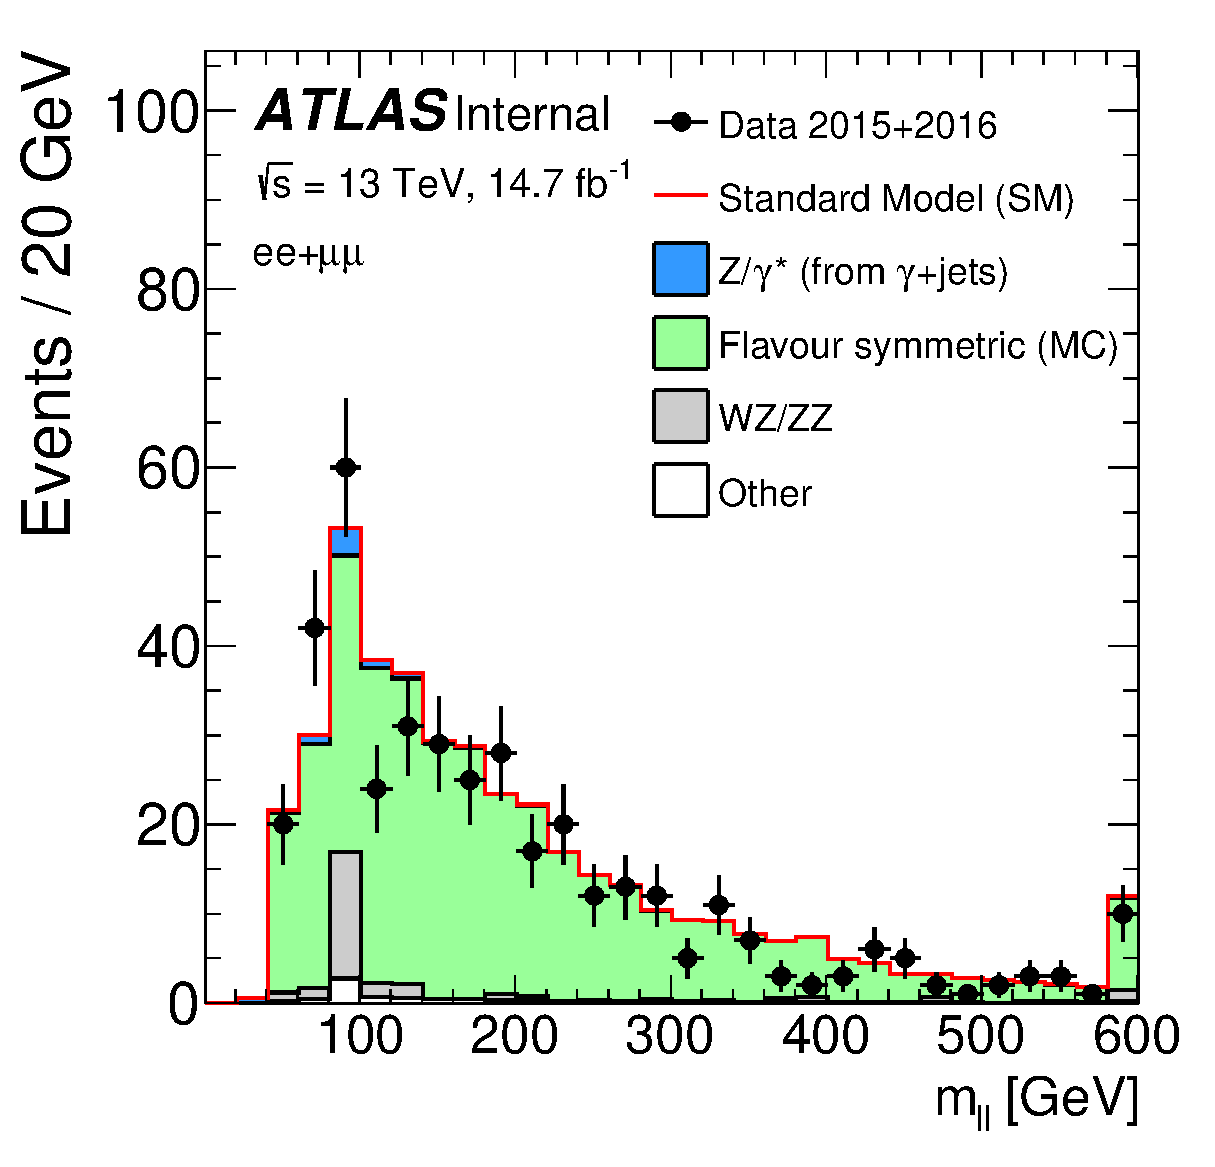
\includegraphics[width=.48\linewidth]{figures/results/mll_SF_R_a_SCALED.eps}
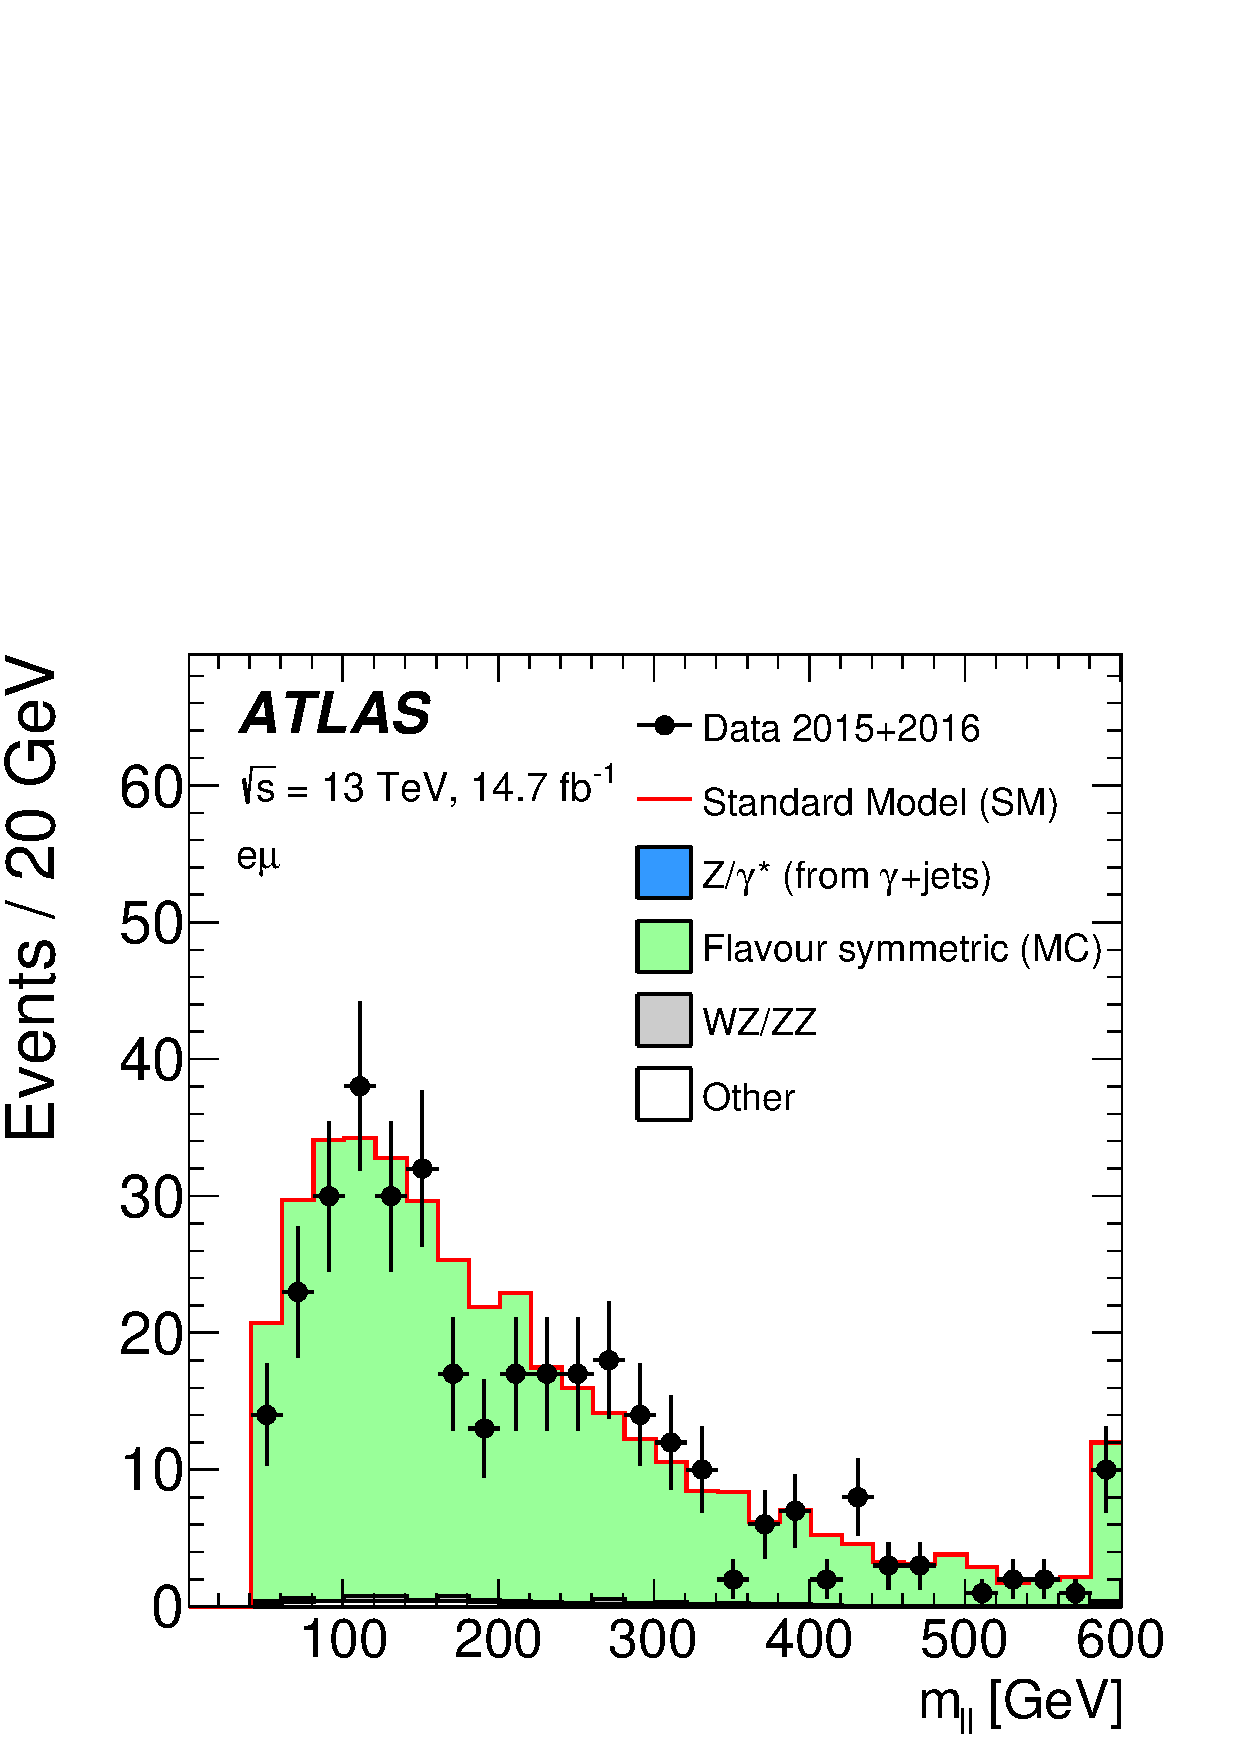
\includegraphics[width=.48\linewidth]{figures/results/mll_DF_R_a_SCALED.pdf}
\caption{Comparisons as a function of \mll~of background predictions with observed data in an SRZ-like region, with the \mll~cut removed. Left is the same-flavor channel, where all background shapes are taken from \ac{MC} and scaled to their SRZ predictions, except for the \dyjets background, which is taken entirely from the data-driven background. Right is the different-flavor channel, in which the backgrounds are taken directly from \ac{MC}, except for \ttbar, which is scaled to match the total data yield. }
\label{fig:results_widemll}
\end{figure}
\end{centering}

Focusing in on the \ac{SR} itself, comparisons of background predictions, observed events, and signal models can be made as a function of key variables for the analysis. \autoref{fig:results_srdists} shows several of these. The first two figures focus on the features of the \ac{SR} events' leading leptons; they give the mass and \pt of a hypothetical parent particle reconstructed from the leptons. In the case of events with a real $Z$ boson, these variables simply give that boson's mass at \pt. The next two figures show distributions in the two most important variables used to differentiate signal from background, \met and \HT. In this analysis, where the frozen \ac{SR} resulted in cuts on these quantities that are lower than those that would be chosen based on a new optimization, these plots show that, even in more sensitive regions, no large excess above the \ac{SM} background is seen. The last pair of figures relates to the jets in the event, showing the total number of jets and the total number of $b$-jets in the \ac{SR} events. The $b$-jet quantity is not explicitly cut on in the analysis because the fraction of $b$-jets produced is extremely model dependent. However, an excess at high $b$-jet multiplicity would suggest a \ac{BSM} process. In each of these distributions, the observed distributions match the background predictions very well, and no evidence for any of the superimposed signal models is seen. 

\begin{centering}
\begin{figure}[!hbt]
\myfloatalign
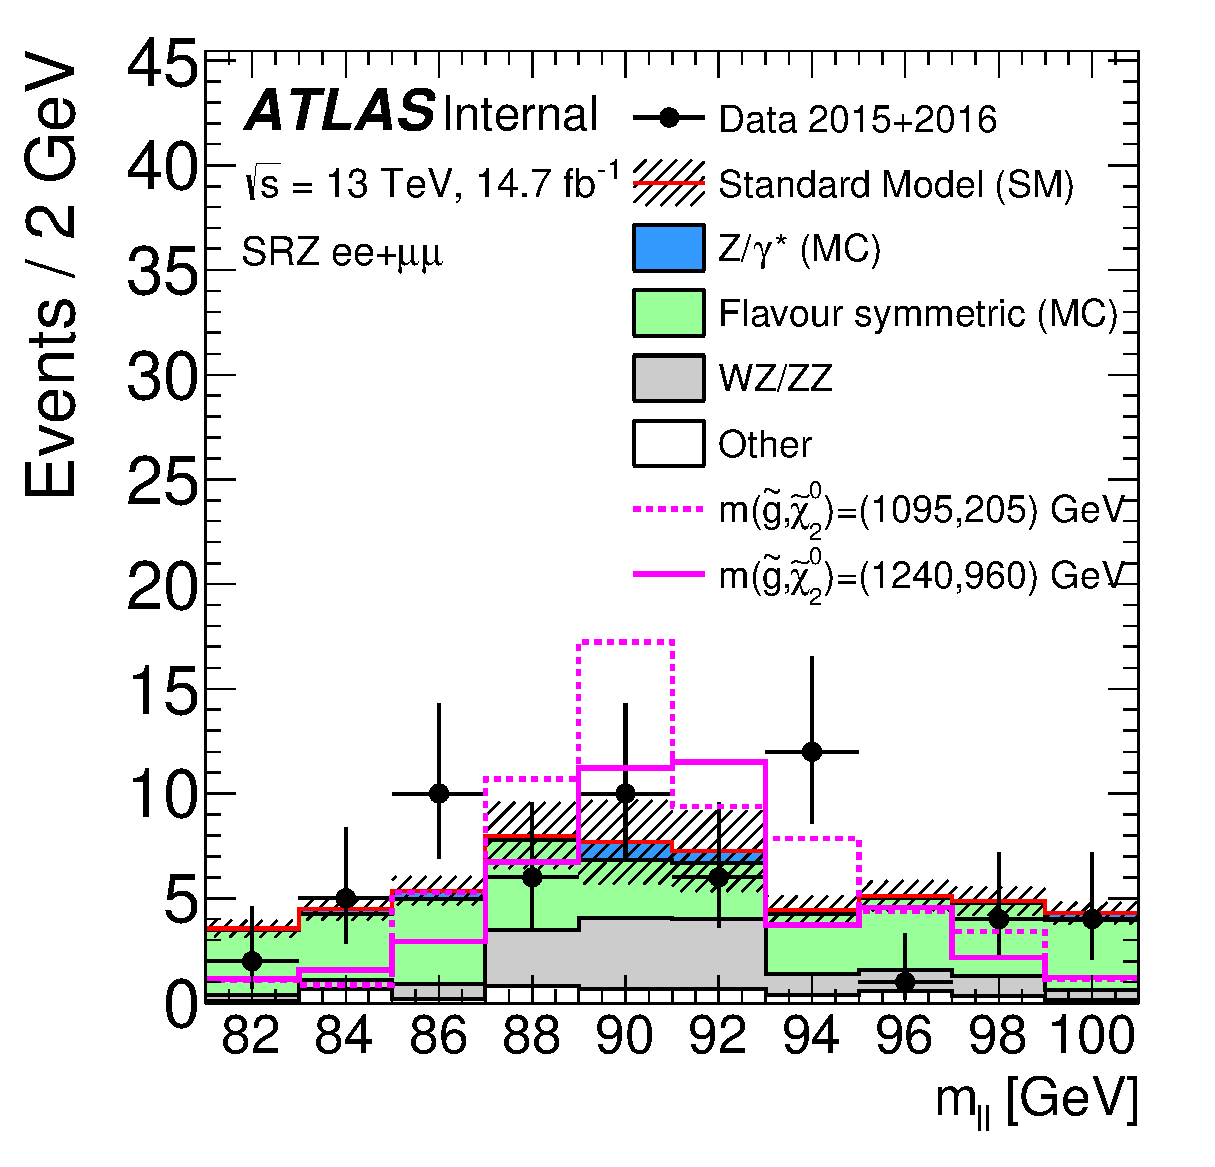
\includegraphics[width=.48\linewidth]{figures/results/mll_ee_mm_srz_R_a.eps}
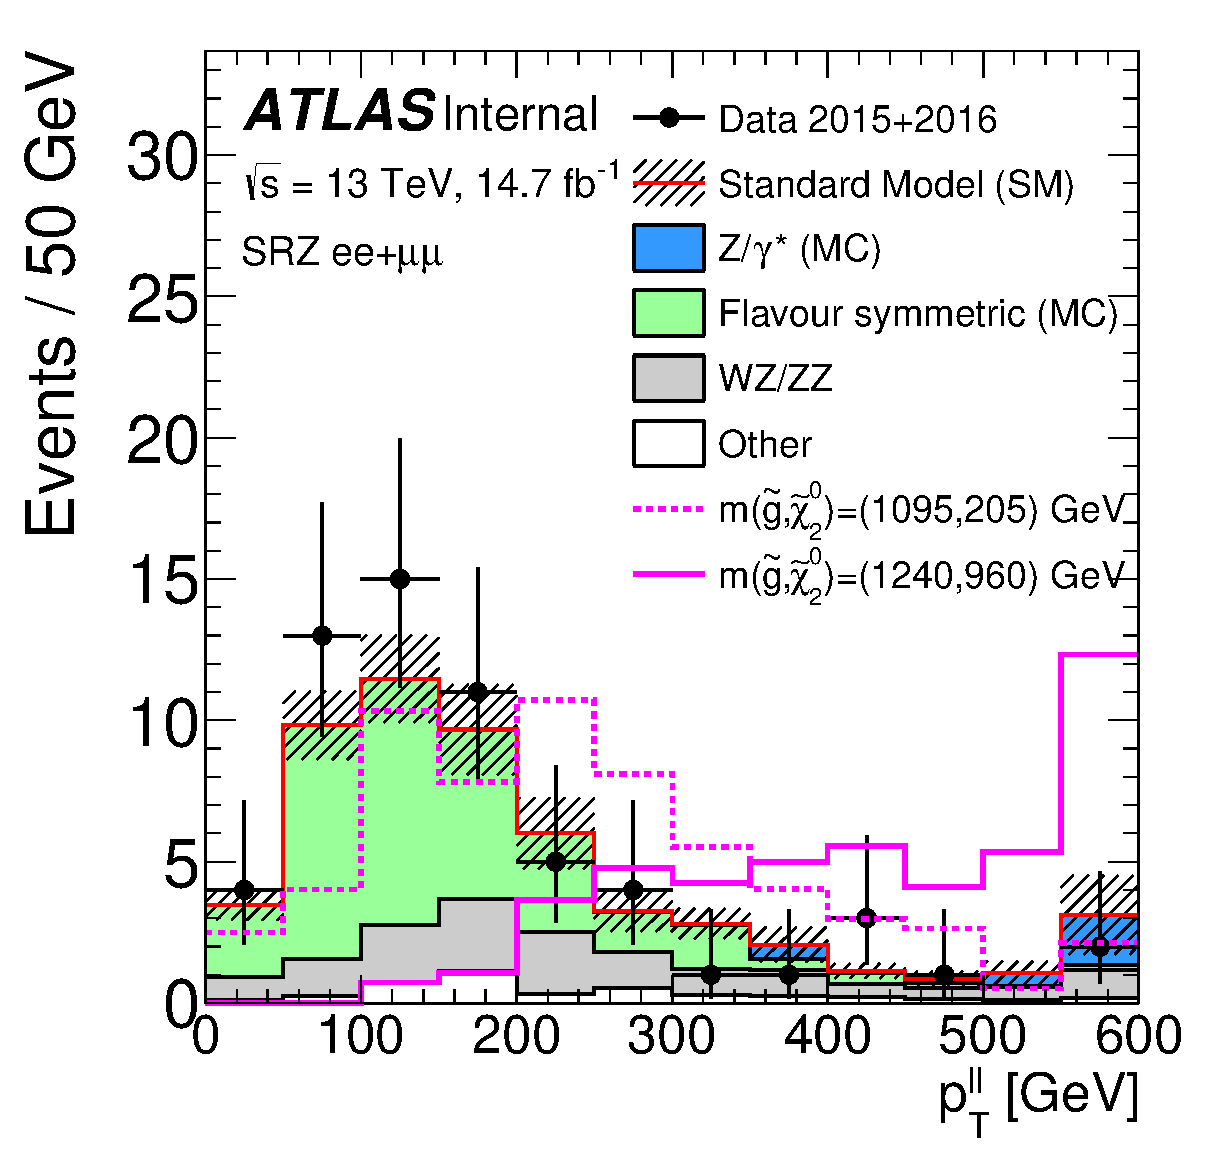
\includegraphics[width=.48\linewidth]{figures/results/Zpt_ee_mm_srz_R_a.eps}
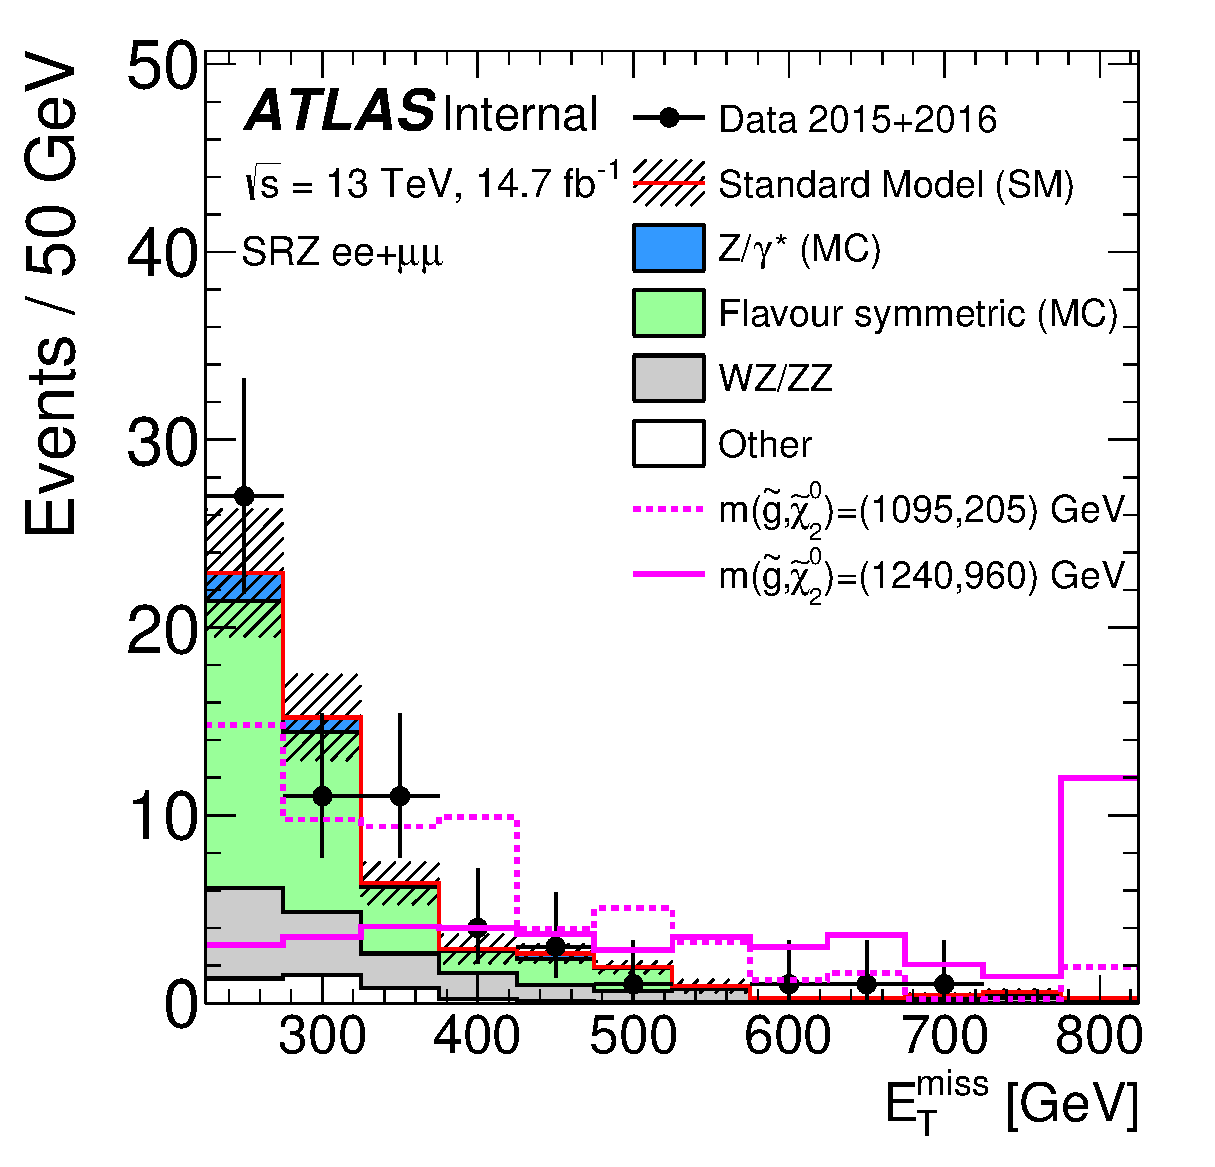
\includegraphics[width=.48\linewidth]{figures/results/met_ee_mm_srz_R_a.eps}
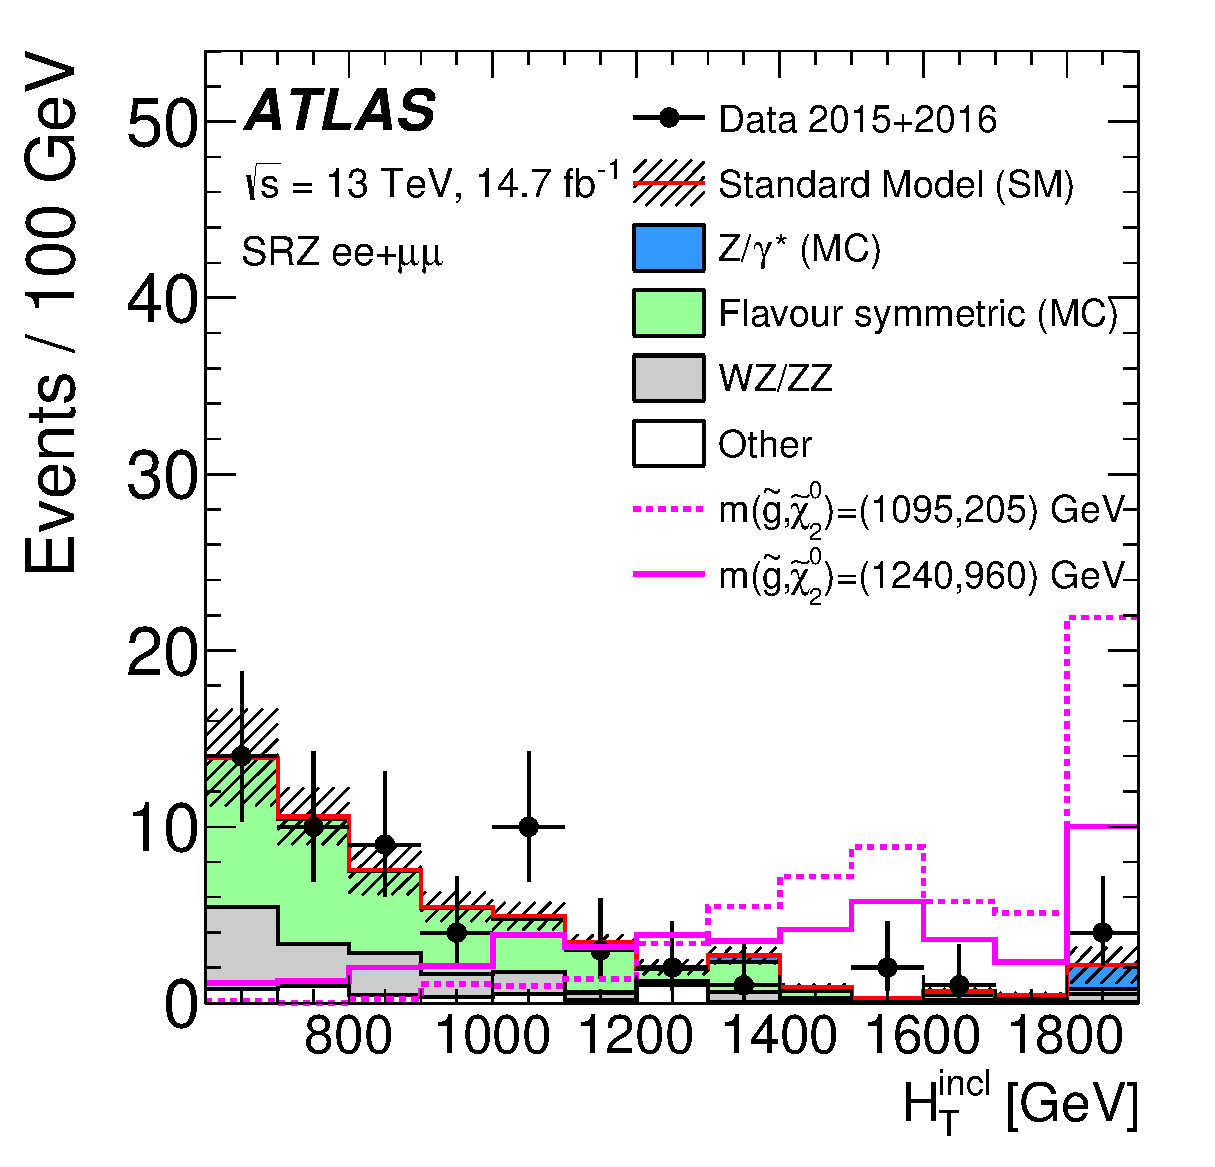
\includegraphics[width=.48\linewidth]{figures/results/htincl_ee_mm_srz_R_a.eps}
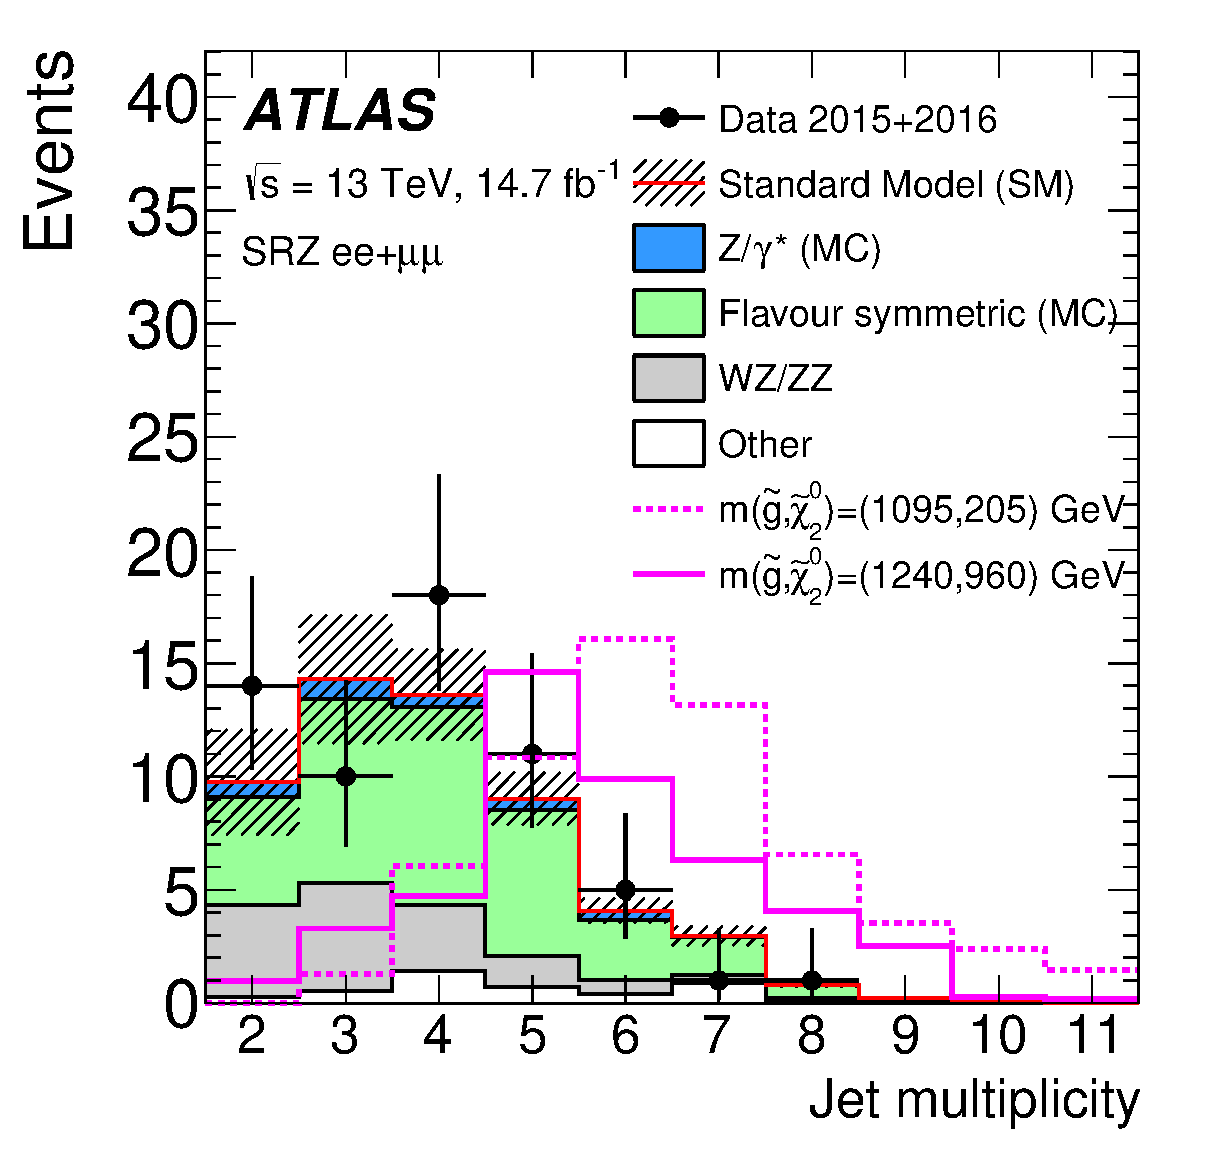
\includegraphics[width=.48\linewidth]{figures/results/njets_ee_mm_srz_R_a.eps}
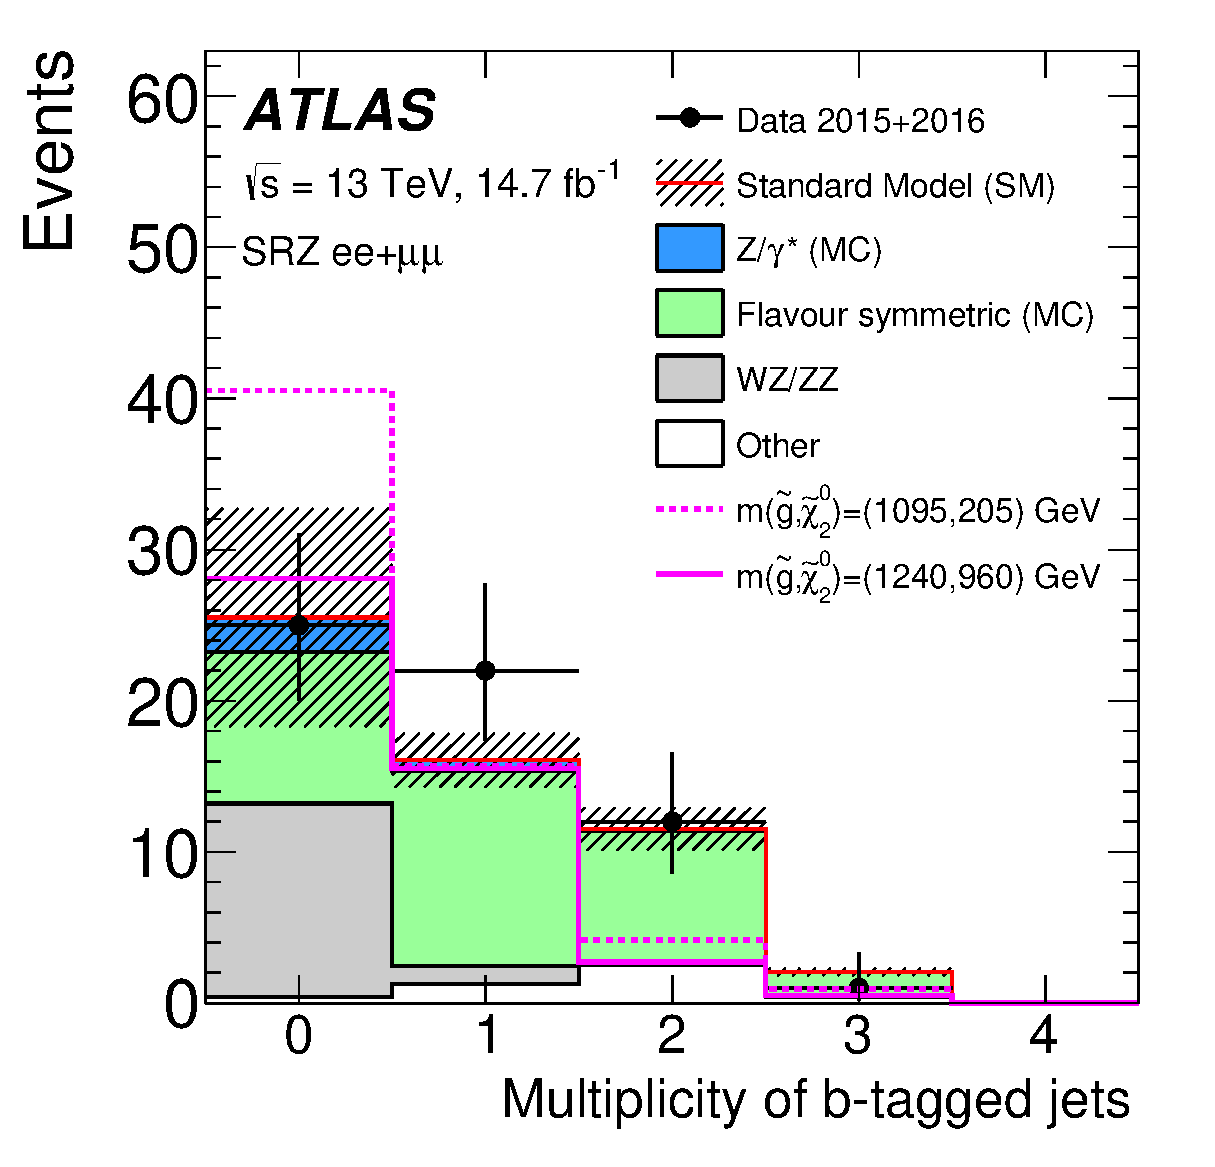
\includegraphics[width=.48\linewidth]{figures/results/nbjets_ee_mm_srz_R_a.eps}
\caption{ Distributions of observed data, background predictions, and simulated signals are shown in SRZ as a function of \mll, $\pt^{\ell\ell}$, \met, \HT, number of jets, and number of $b$-jets. The two example signals have $(m(\tilde{g}),m(\tilde{\chi}^{0}_{2}))=(1095, 205)$~\GeV. All background shapes are taken from \ac{MC}, and in the case of flavor symmetric and \dyjets backgrounds, their yields are scaled to match the data-driven predictions. Uncertainties include statistical and systematic components.}
\label{fig:results_srdists}
\end{figure}
\end{centering}

Comparisons of the observed and expected yield are also made as a function of $\Delta\phi(\text{jet}_{12},{\boldsymbol p}_{\mathrm{T}}^\mathrm{miss})$, shown in \autoref{fig:results_dphi}. Here, results are shown in a region similar to SRZ with the cut on this variable removed, showing the efficacy of the background prediction in a region enhanced in \dyjets events. Again, excellent agreement is seen between the background prediction and observed data.

\begin{centering}
\begin{figure}[!hbt]
\myfloatalign
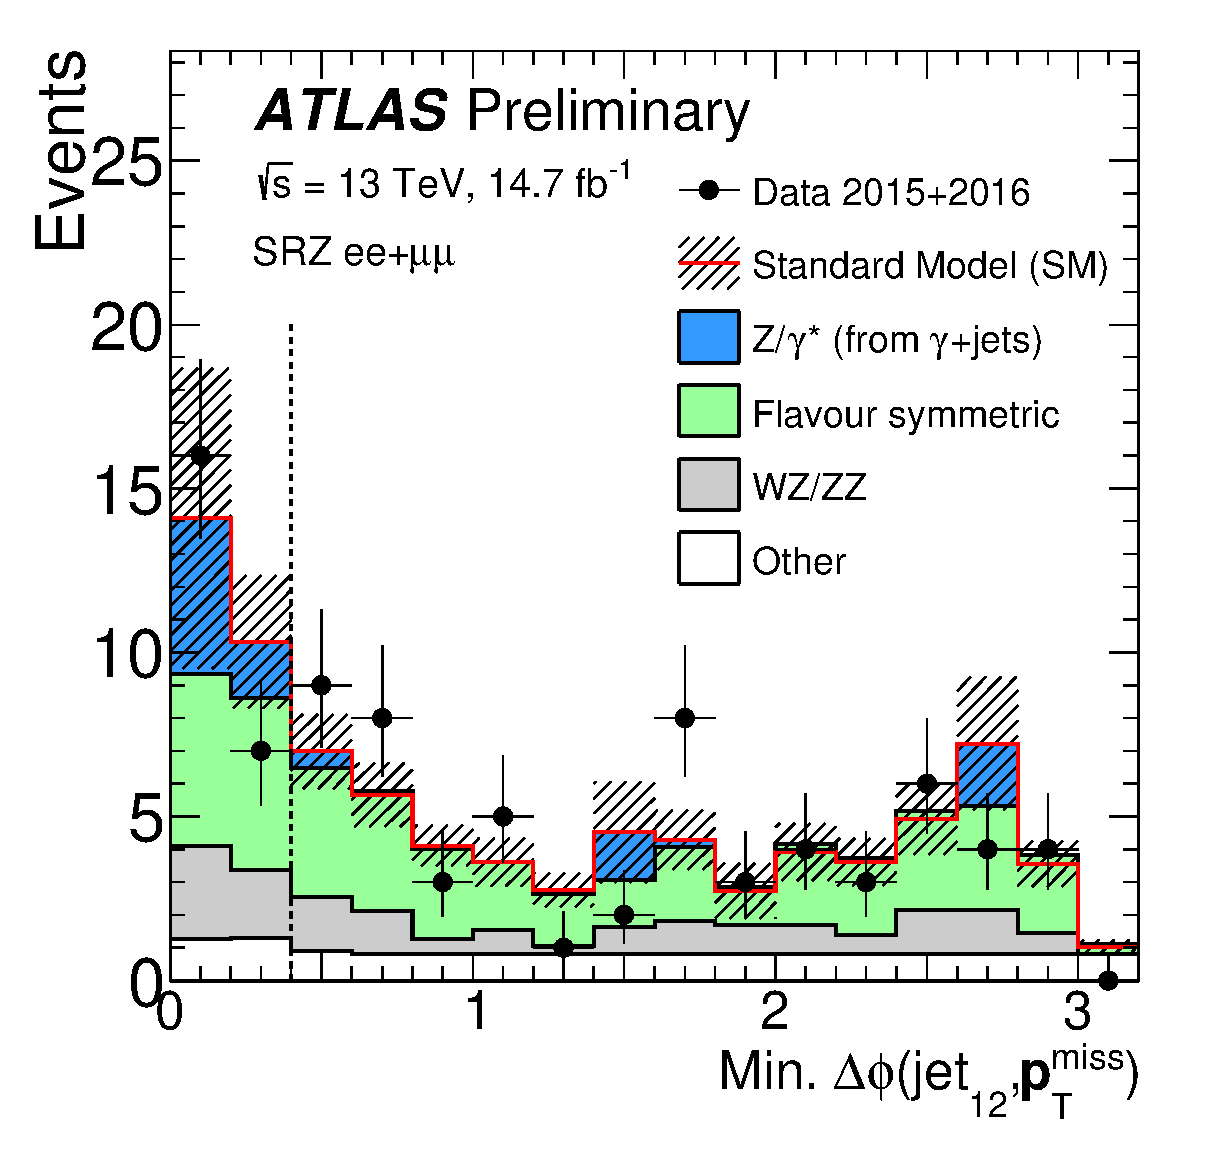
\includegraphics[width=.9\linewidth]{figures/results/dPhi_azmet_ee+mm_onz_SR.eps}
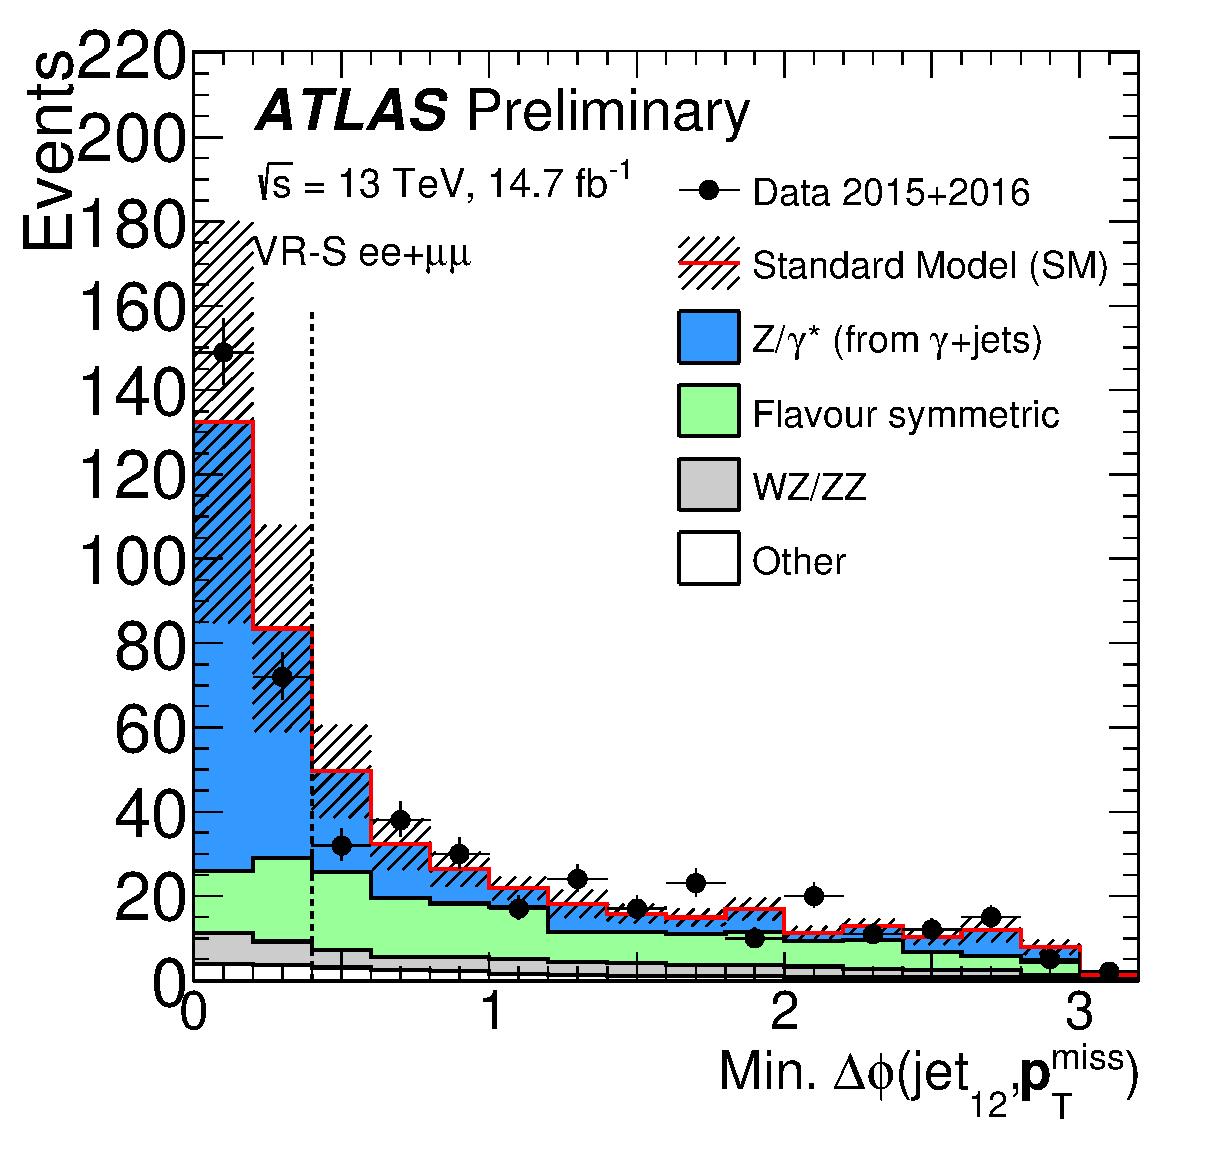
\includegraphics[width=.9\linewidth]{figures/results/dPhi_azmet_ee+mm_onz_VR.eps}
\caption{Comparisons as a function of $\Delta\phi(\text{jet}_{12},{\boldsymbol p}_{\mathrm{T}}^\mathrm{miss})$ of background predictions with observed data in an SRZ-like (left) and VRS-like (right) region, with the $\Delta\phi(\text{jet}_{12},{\boldsymbol p}_{\mathrm{T}}^\mathrm{miss})$ cut removed. All background shapes are taken from \ac{MC} and scaled to their SRZ predictions, except for the \dyjets background, which is taken entirely from the data-driven background.}
\label{fig:results_dphi}
\end{figure}
\end{centering}

%----------------------------------------------------------------------------------------
